\chapter{Design af brugergrænsefladen}
\label{Design_G}
Dette kapitel beskriver brugergrænsefladen samt de beslutninger, som ligger bag. Alle vores papermockups og endelige skærmbilleder findes i appendix \ref{App_GUI}.

\section{Brugergrænsefladens udvikling og udseende}
\label{Design_G_Development}
\begin{figure}[h!]
  \centering
    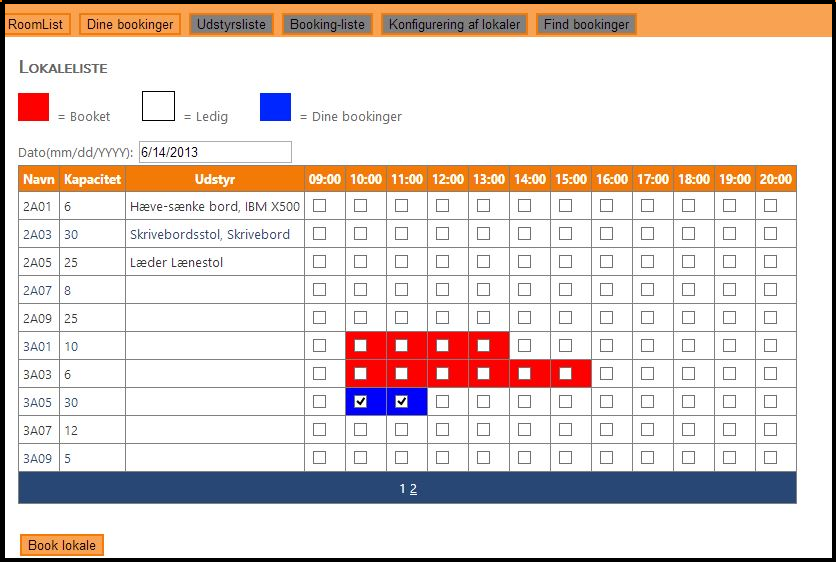
\includegraphics[width=0.7\textwidth]{Appendix/GUI-Prototype/DigitalMockup/GridEksempel}
  \caption{Skærmbilledet til booking af lokaler}
\label{Design_G_Development_FinalGrid}
\end{figure}

Vores skærmbilleder er opdelt i tre typer: Gitter, Almindelig og Pop-ups. 
\\Gitterskærmbillederne bruger vi til booking af lokale, forplejning og udstyr samt administration af bookinger, lokaleinventar og udstyr.
\\Almindelige vinduer anvender vi i forbindelse med login eller, hvis man skal ændre noget på et stykke udstyr/inventar.
\\Pop-up skærmbilleder er generelt advarsler eller fejlbeskeder.

Det første skærmbillede man ser, når man starter programmet er en liste over lokaler, som viser, hvilke tidspunkter lokalerne er ledige.
\\For at booke et lokale markerer man tiderne i checkboksene, der hører til det ønskede lokale og trykker "Book lokale". Hvis man ikke er logget ind, bliver man redirected til login skærmbilledet.
\\Det har været vores mål, at brugeren skal have adgang til så meget information, som det er muligt at give, uden at brugeren logger ind.

\begin{figure}[h!]
  \centering
    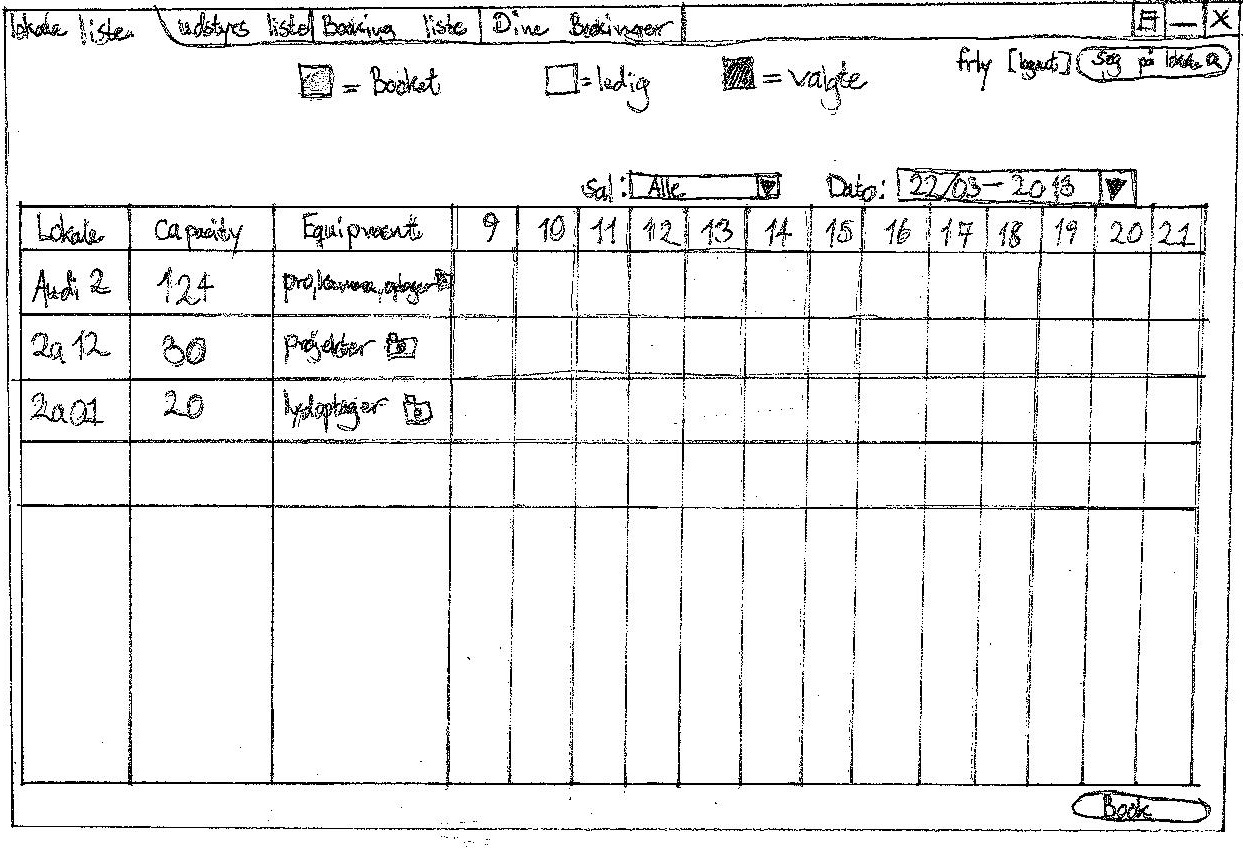
\includegraphics[width=0.9\textwidth]{Appendix/GUI-Prototype/PaperMockup/LokaleListe_001}
  \caption{Første udgave af gitter layoutet}
\label{Design_G_Development_FirstGrid}
\end{figure}

Vores første mockup af skærmbilledet til booking af lokaler (figur \ref{Design_G_Development_FirstGrid}) havde et gitter, hvor hver række var et lokale og tiderne var kolonner. Man skulle klikke i et felt for at vise, at man ønskede at booke på et bestemt tidspunkt. Usability test viste dog, at det ikke var en intuitiv måde at vælge tidspunkter på, så vi tilføjede checkbokse til gitteret.
Figur \ref{Design_G_Development_FinalGrid} viser den endelige version.

\begin{figure}[h!]
  \centering
    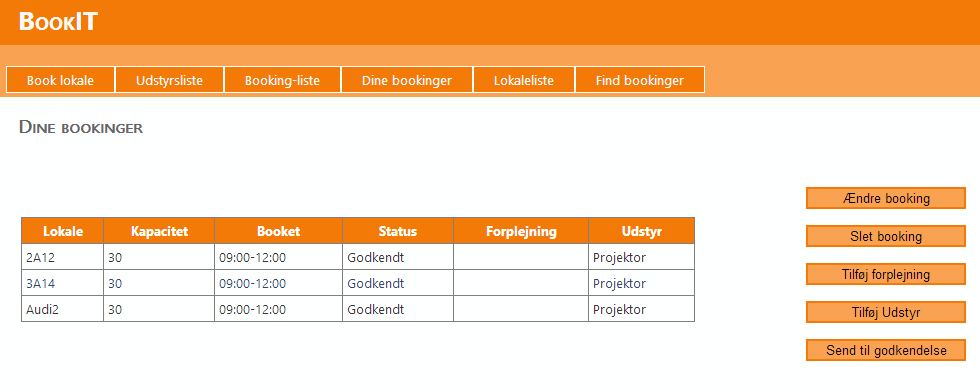
\includegraphics[width=0.7\textwidth]{Appendix/GUI-Prototype/DigitalMockup/DineBookinger}
  \caption{Skærmbilledet til visning af bookinger}
\label{Design_G_Development_YourBookings_Final}
\end{figure} 

Når man har valgt lokale og tidspunkt, trykker man "Book lokale". Dette sender en til skærmbilledet "Dine Bookinger", som viser en liste over ens egne bookinger (se figur \ref{Design_G_Development_YourBookings_Final}). 
\\Hvis man vælger en booking og trykker "Ændre Booking", navigeres der til lokalelisten, hvor man kan ændre sin booking ved at tilføje/fjerne markeringer i checkboksene. 
\\Hvis man i stedet trykker "Tilføj Forplejning" bliver man sendt til forplejningsskærmbilledet.

\begin{figure}[h!]
  \centering
    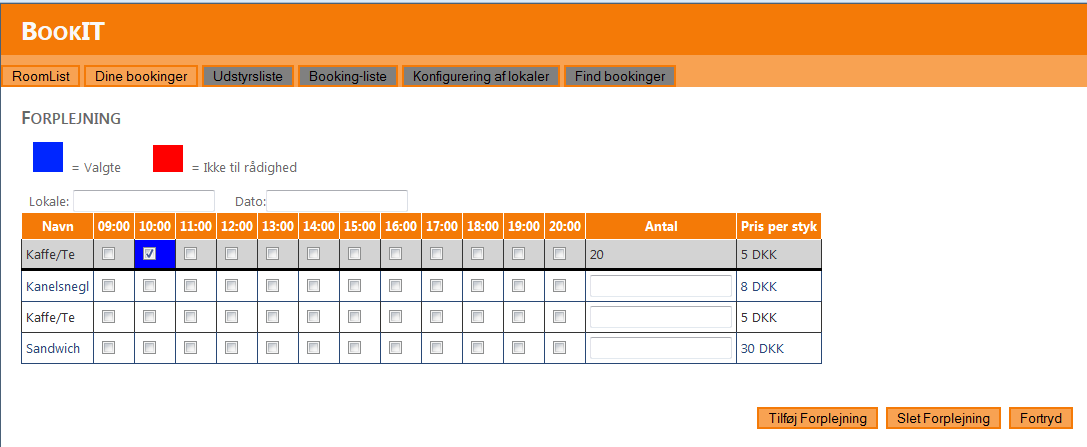
\includegraphics[width=0.85\textwidth]{Appendix/GUI-Prototype/DigitalMockup/Forplejning}
  \caption{Skærmbilledet til booking af forplejning}
\label{Design_G_Development_Forplejning_Final}
\end{figure} 

Figur \ref{Design_G_Development_Forplejning_Final} viser det endelige skærmbillede til valg af forplejning. For at tilføje forplejning til en booking skal man markere den tid, man gerne vil have forplejningen leveret samt angive, hvor mange/meget af forplejningstypen, man gerne vil bestille.
\\Vi fokuserede på at designe skærmbilledet på samme måde, som vi havde designet lokalelisten. Det samme gælder for skærmbilledet til tilføjelse af udstyr til en booking (se figur \ref{App_GUI_final_BookEquip} i appendix).

\subsection{Bookingliste}
Man kan i skærmbilledet til booking liste kan administratoren makere booking i listen og enten godkend eller afvis brugerens booking ved at markere den og trykke på "Godkend" eller "Afvis" knapperne.
Figur \ref{Design_G_Development_BookingListe} viser vores papermockup til godkendelse af bookinger. 
I papermockup havde vi godkend/afvis-knapperne inde i selve gitteret. Dette besluttede vi dog kunne blive forvirrende, så den endelige version af skærmbilledet (figur \ref{Design_G_Development_BookingListe_Final}) har knapperne ved siden af gitteret. Da ingen af de andre skærmbilleder har egentlige knapper inde i gitteret, opfylder i større grad reglen om få vindueskabeloner.

\begin{figure}[h!]
  \centering
    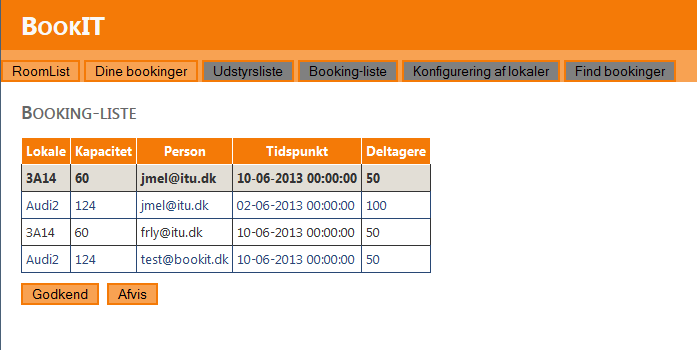
\includegraphics[width=0.7\textwidth]{Appendix/GUI-Prototype/DigitalMockup/BookingListe}
  \caption{Skærmbilledet af recepcionistens liste af bruger bookinger}
\label{Design_G_Development_BookingListe_Final}
\end{figure} 

\begin{figure}[h!]
  \centering
    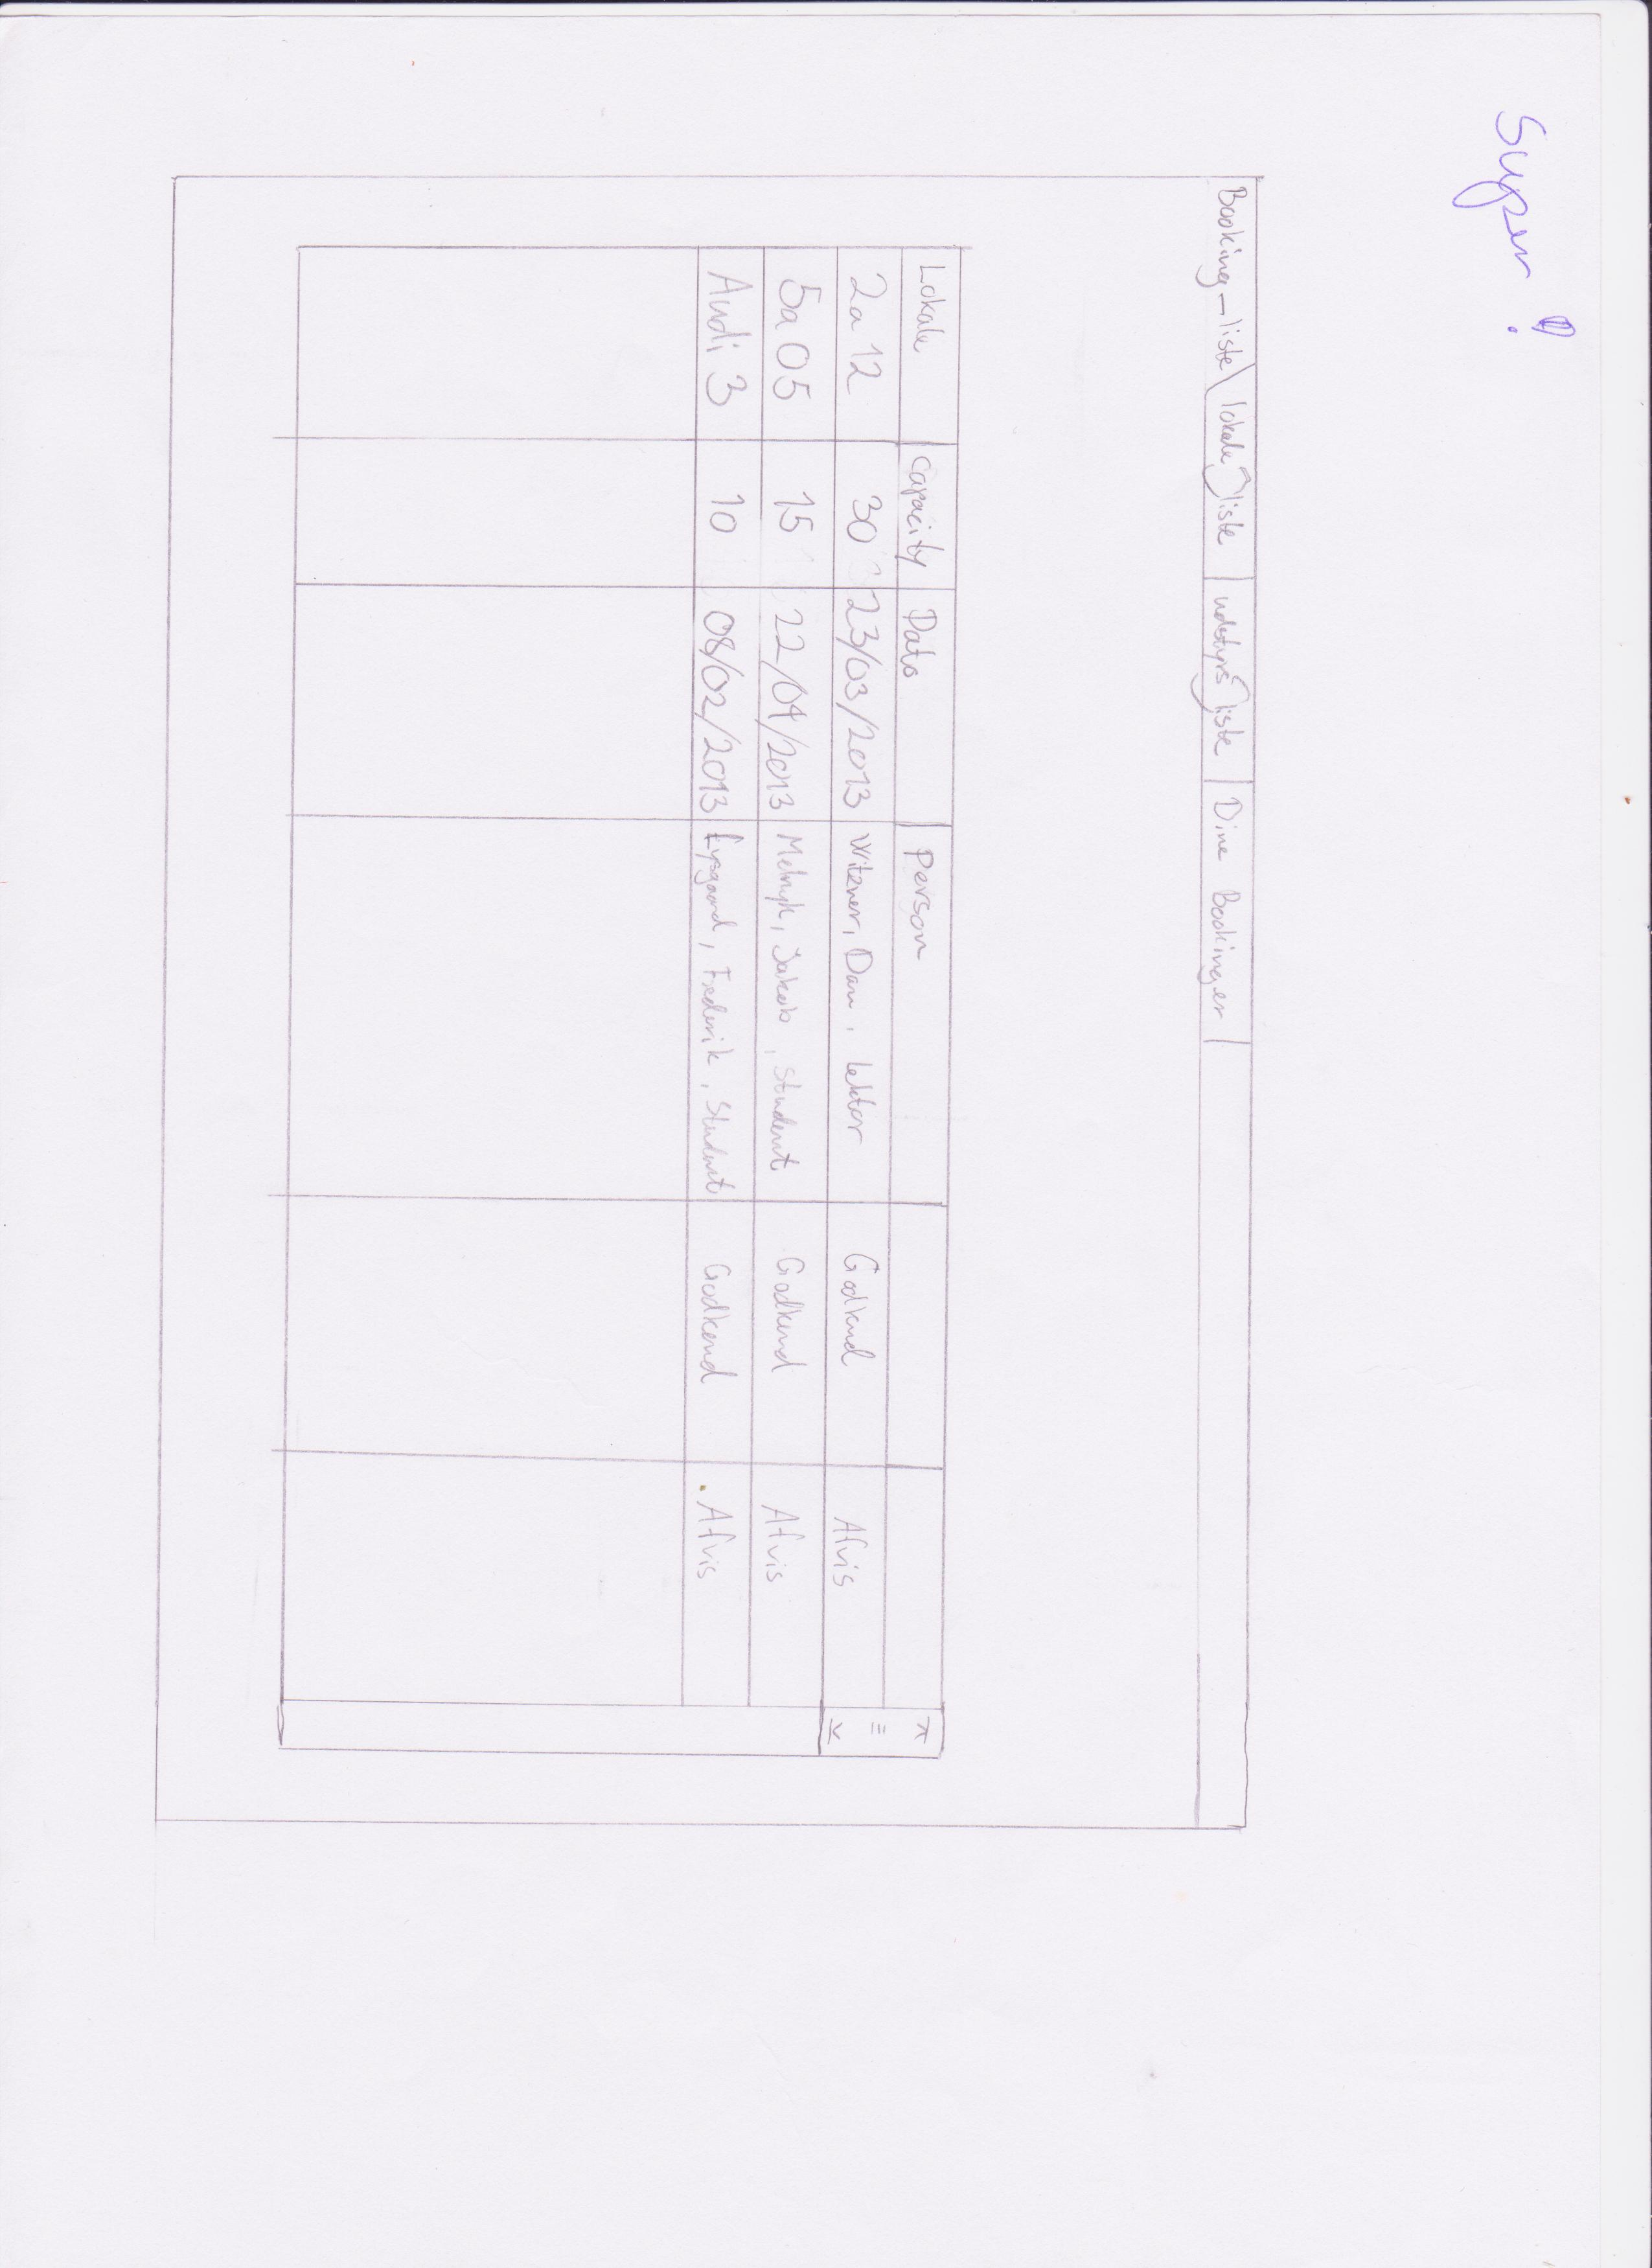
\includegraphics[width=0.7\textwidth]{Appendix/GUI-Prototype/PaperMockup/GodkendBookinger_001}
  \caption{Papermockup af recepsionistens liste af bruger bookinger}
\label{Design_G_Development_BookingListe}
\end{figure} 

\subsection{Udstyrsliste}
I skærmbilledet over udstyrslisten kan man i venstre side se en liste over det udstyr der allerede er i systemet, hvis man vil ændre eller slette noget af det vælger man udstyret og trykke på "Ændre Udstyr" eller "Slet Udstyr" knappen. Højre side af skærmbilledet giver brugeren mulighed for at tilføj lokaler til listen på venstre side ved at udfylde felterne med data og trykke på "Tilføj udstyr".

Figur \ref{Design_G_Development_UdstyrsListe_Final} viser det endelige skærmbillede af listen over udstyr.
Skærmbilledet indeholder både overblikket over alt det udstyr, som er tilrådighed, og muligheden for at registrere nyt udstyr til systemet.
\\Vi delte de to funktionaliteter op, så det var tydeligt, at det er seperate funktionaliteter.

Den eneste ændring siden vores papermockup (se appendix) er tilføjelsen af en checkbox, hvor man kan vælge et nyt stykke udstyr skal være til udlån. Dette betyder, at vi sparer et skærmbillede væk. Da udstyr og inventar er stort set ens i systemet, kan vi afgøre, om det nye element er inventar eller udstyr gennem denne checkbox.

\begin{figure}[h!]
  \centering
    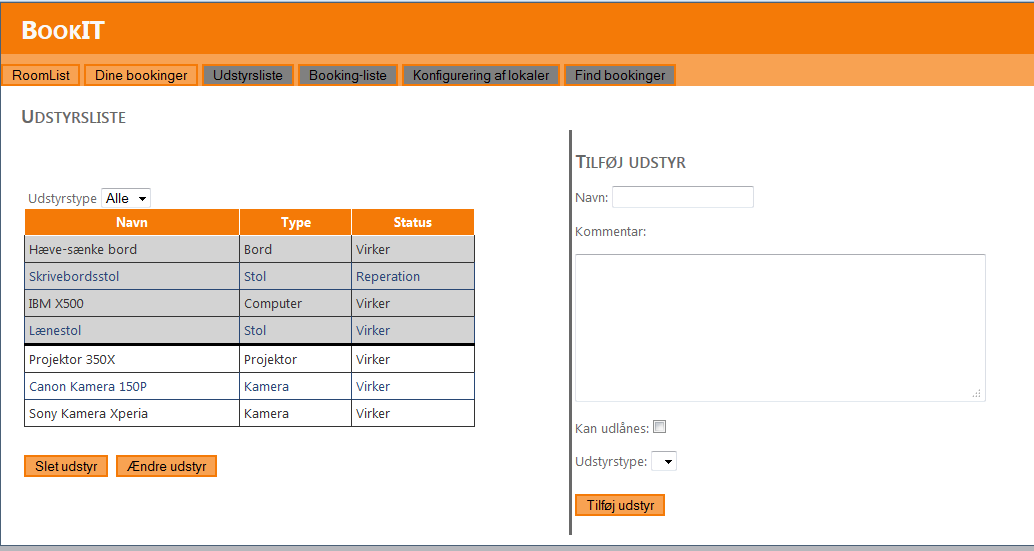
\includegraphics[width=0.7\textwidth]{Appendix/GUI-Prototype/DigitalMockup/UdstyrsListe}
  \caption{Skærmbilledet af recepsionistens liste over udstyr i ITUs system.}
\label{Design_G_Development_UdstyrsListe_Final}
\end{figure} 

\subsection{Ændring af lokale}
I" Ændring af lokale" er det muligt for administateren at ændre navnet på et lokale samtidig med at man kan fjerne eller tilføje udstyr ved at markere det i listen og bruge knappen "Tilføj udstyr" som vil skifte tekst til "Slet udstyr" hvis man markere udstyr der allerede er i lokalet.
Skærmbilledet er designet således, at man kan ændre navn og kapacitet på lokalet samtidig med, at man kan få et overblik over udstyret, som er tilføjet til lokalet.

Papermockup af dette skærmbillede (figur \ref{Design_G_Development_AendreLokale}) var delt op i tre dele: et til at skifte navn/kapacitet, et til at tilføje inventar og et til at fjerne inventar.
\\Dette var meget uoverskueligt og mindede ikke om resten af vores design. Vi valgte derfor at bruge gitterløsningen til udstyret. Den øverste del af gitteret viser det inventar, som er tilføjet lokalet. Resten af gitteret viser det inventar, som ikke er tildelt noget lokale. Teksten på "Tilføj Udstyr"-knappen ændrer sig til "Fjern Udstyr", hvis man trykker på en linje i den øverste del af gitteret.

\begin{figure}[h!]
  \centering
    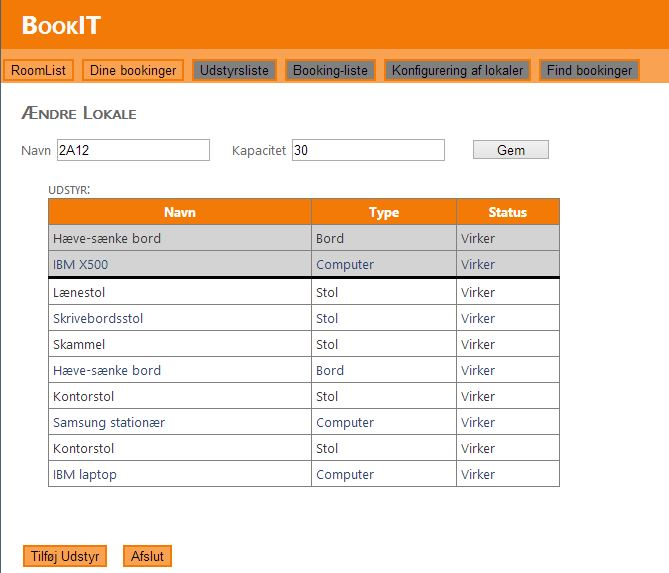
\includegraphics[width=0.7\textwidth]{Appendix/GUI-Prototype/DigitalMockup/AendreLokale}
  \caption{Skærmbilledet til ændring af lokale.}
\label{Design_G_Development_AendreLokale_Final}
\end{figure} 

\clearpage
\begin{figure}[h!]
  \centering
    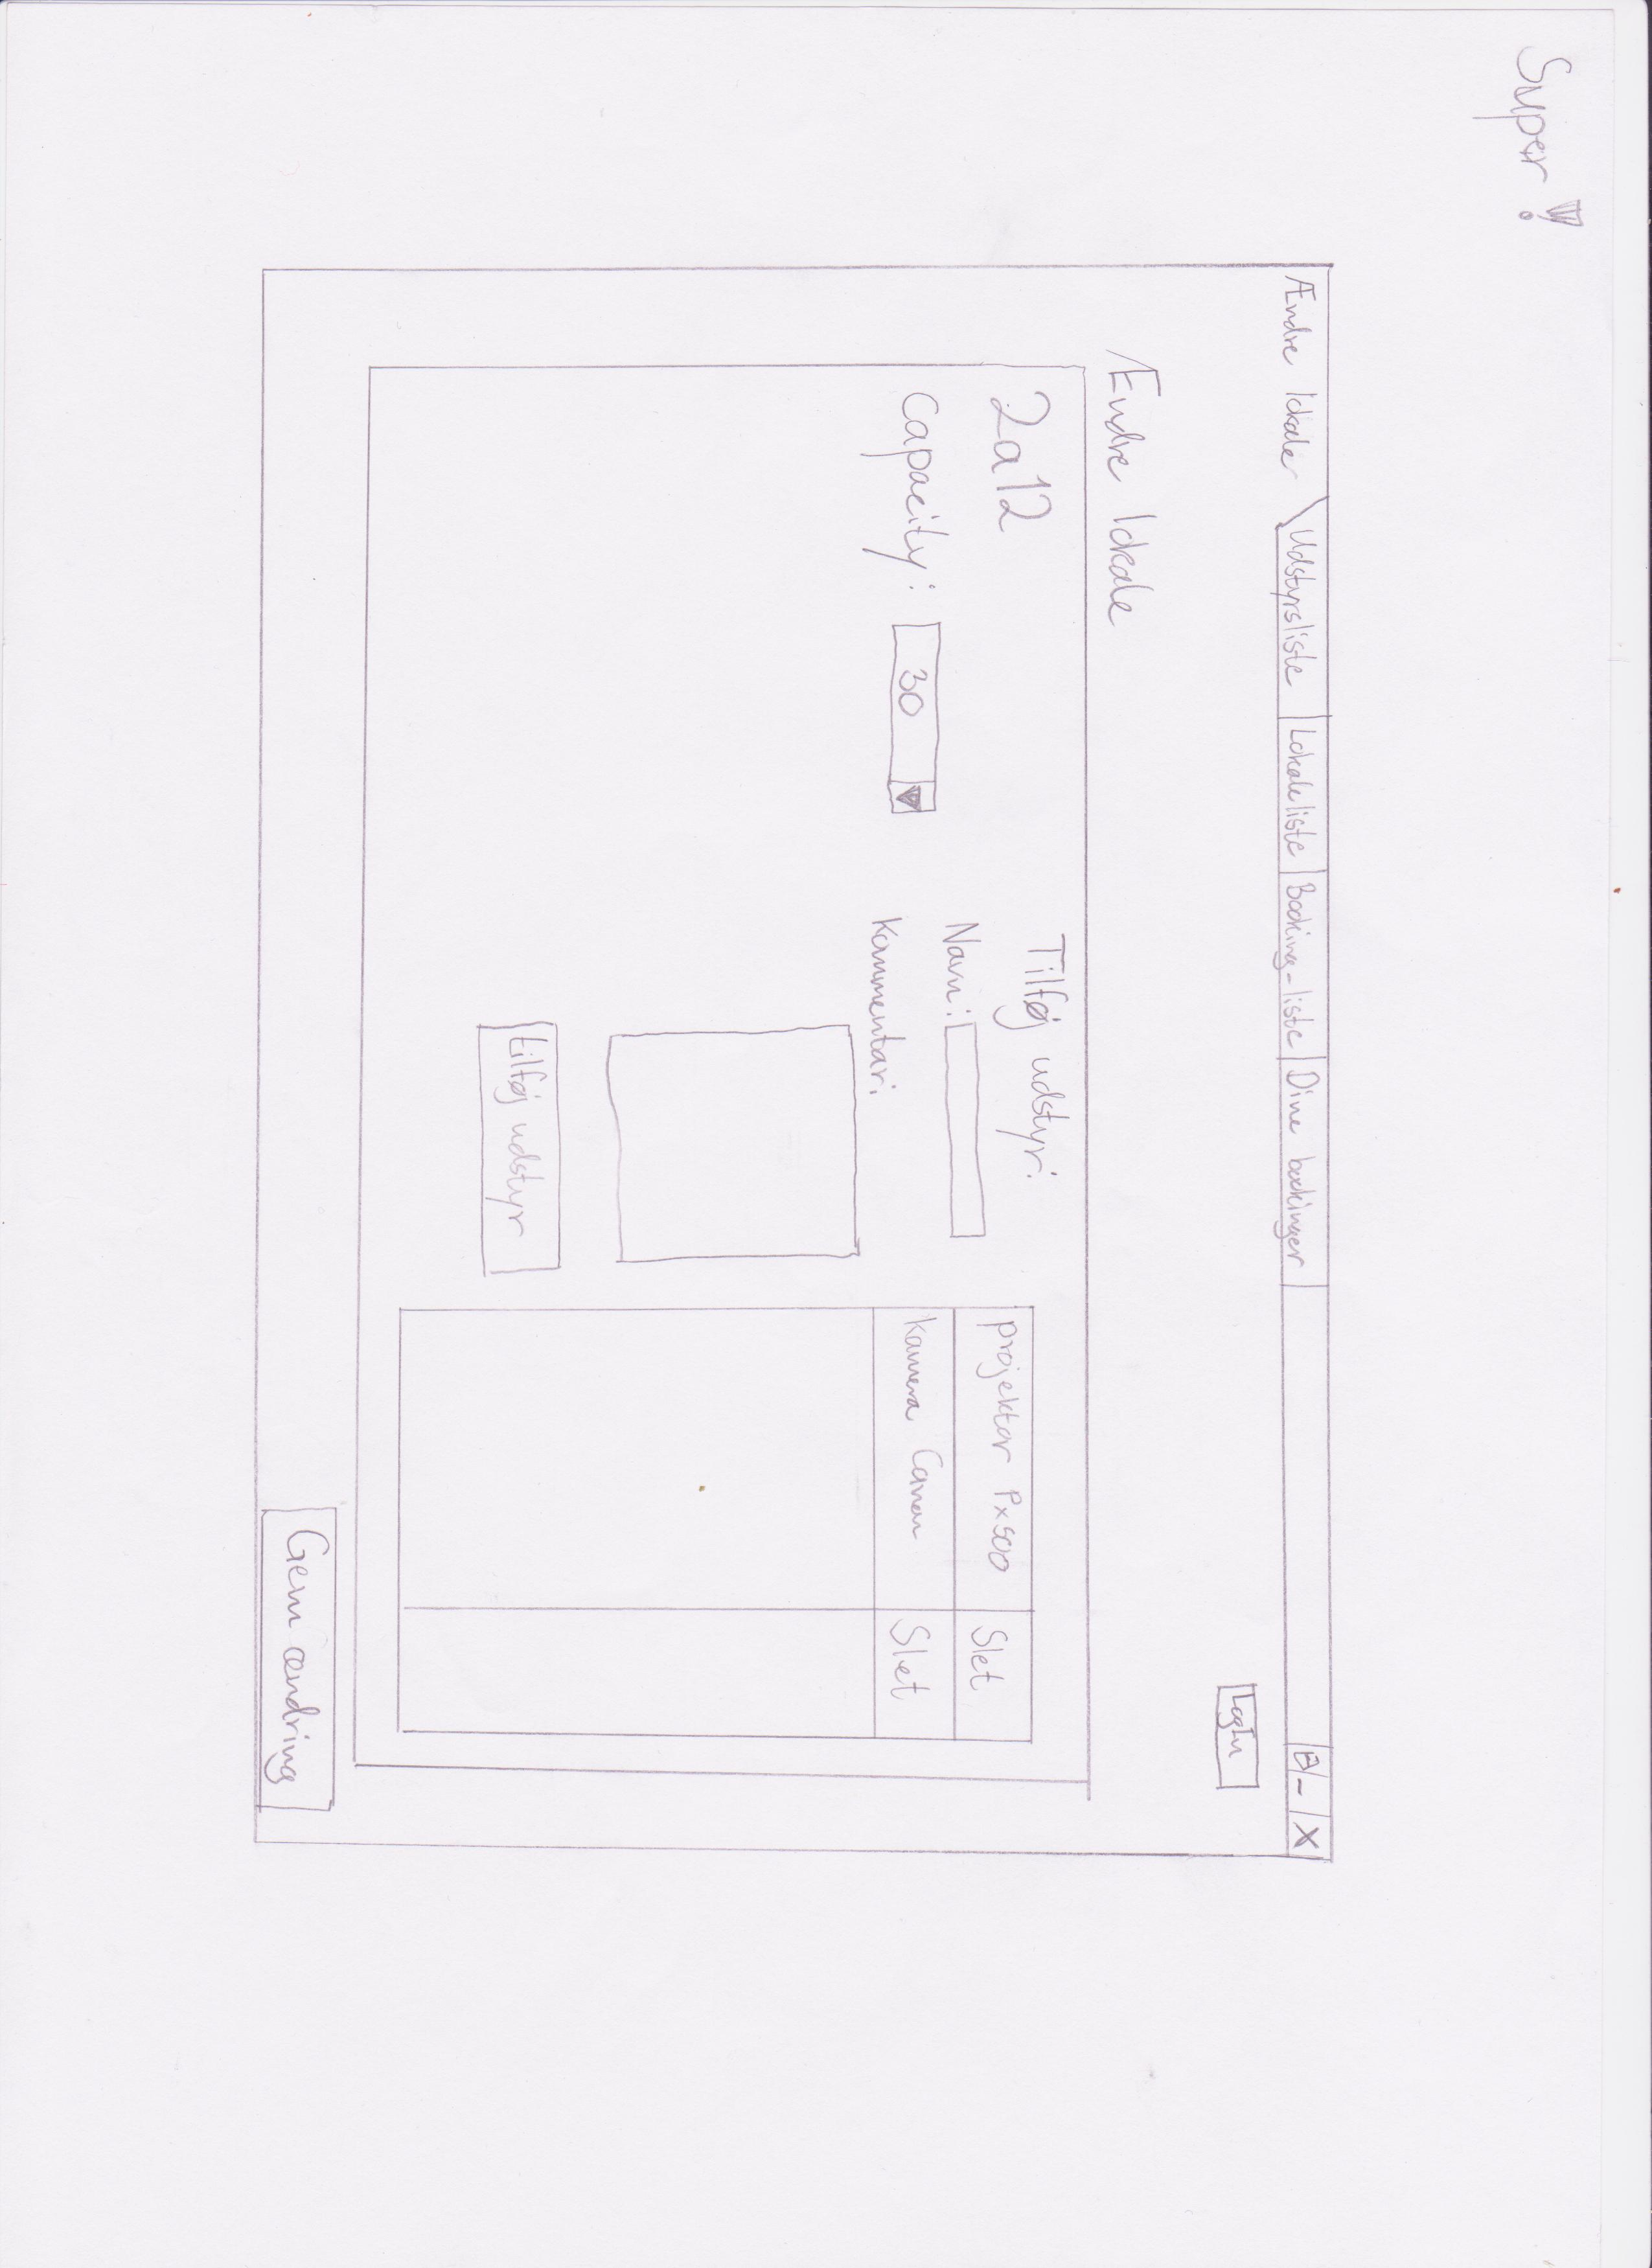
\includegraphics[, width=0.7\textwidth]{Appendix/GUI-Prototype/PaperMockup/AendreLokale_001}
  \caption{Papermockup til ændring af lokale.}
\label{Design_G_Development_AendreLokale}
\end{figure} 

\section{Generelle mål}
\label{Design_G_Goals}
Vi har valgt at designe vores brugergrænseflade ud fra reglerne om design af virtuelle vinduer\cite[s. 169]{SL_UID} samt Ease Of Use principperne\cite[s. 9]{SL_UID}. I forbindelse med dette valg har vi sat følgende mål for designet:
\begin{itemize}
\item Konsistent brugergrænseflade
\item Få forskellige skærmbilleder
\item Overblik
\item Effektivt
\end{itemize}

\subsection{Konsistent brugergrænseflade}
Vi har valgt at designe skærmbillederne med samme grundstruktur. Denne lighed bør gøre det intuitivt at gå fra et skærmbillede til et andet i forbindelse med udførsel af opgaver. Desuden følger det reglen om få vindueskabeloner.

\subsection{Kort vej fra en opgave til en anden}
Brugergrænsefladen skal gøre det hurtigt og nemt for brugeren at komme fra en opgave til en anden. Dette skal gøres ved at have få skærmbilleder involvereret i en enkelt task (reglen om få vinduer per opgave).

\subsection{Overblik}
Brugeren skal have mulighed for nemt at danne sig overblik over bookinger, udstyr og forplejning\footnote{Reglen om den nødvendige oversigt af data.}. Derfor skal vi have seperate skærmbilleder, som giver overblik over hver type.

\subsection{Effektivt}
Det skal være effektivt at udføre opgaver for brugere, som anvender systemet ofte.